% !Mode:: "TeX:UTF-8"
\chapter{Java基础}

\begin{introduction}
	\item 变量和类型
	\item 输入和输出
	\item 面向对象
	\item 异常处理
	\item 多线程
\end{introduction}

相比于其它编程语言,Java的语法不算多的,很容易掌握。
本章将以最短的篇幅带大家掌握Java编程语言。
编程语言三大核心要素:数据、语句和函数。
数据要先存放在变量中,才能被程序处理,不同类型的变量可存放不同的数据;
需要遍历所有的数据的时候,就会用到\lstinline{for/while}语句;
判断某个条件是否成立,使用\lstinline{if}语句等。
而把常用的逻辑放在一起,就定义了一个函数。

\section{jshell的使用}
本章部分内容,要在jshell(JDK9+)的交互式环境学习验证,请提前配置环境变量。
你可在单台机器上安装多个JDK版本\footnote{DeepLearning4i需要JDK8。},
只要确保你的配置是正确的,就没有关系。

\begin{lstlisting}[language=bash]
	jshell> /help
|  键入 Java 语言表达式, 语句或声明。
|  或者键入以下命令之一:
|  /list [<名称或 id>|-all|-start]
|  	列出您键入的源
|  /save [-all|-history|-start] <文件>
|  	将片段源保存到文件
|  /open <file>
|  	打开文件作为源输入
|  /vars [<名称或 id>|-all|-start]
|  	列出已声明变量及其值
|  /methods [<名称或 id>|-all|-start]
|  	列出已声明方法及其签名
|  /types [<名称或 id>|-all|-start]
|  	列出类型声明
|  /imports 
|  	列出导入的项
|  /exit [<integer-expression-snippet>]
|  	退出 jshell 工具
\end{lstlisting}

使用jshell可以快速验证我们的代码是否正确,并支持类型推断(var)。
下面2个变量定虽然没有设定类型,但根据下一节介绍的规则,可自动推理为int和double类型:
\begin{lstlisting}[language=bash, backgroundcolor=\color{lightgray!10}]
	jshell> var m = 2
	m ==> 2
	jshell> var n = 3.0
	n ==> 3.0
	jshell> /vars
	|    int m = 2
	|    double n = 3.0
\end{lstlisting}

\section{变量和类型}
与其他静态类型语言一样,java支持的基本数据类型有:
\lstinline{boolean、byte、char、short、int、long、float、double}
等。

\begin{table}[!htbp] \centering \small
	\caption{基本数据类型}
\begin{tabular}{|p{1.5cm}|p{3cm}|p{8.5cm}|}
\toprule
	\multicolumn{3}{|c|}{基本类型 - 范围}\\
\midrule
  boolean&1位(4个字节)\footnotemark&true, false \\
	byte&8位(一个字节)&$-128\sim127$\\
	short&16位(两个字节)&$-32768\sim32767$\\
	char&16位(两个字节)&$-32768\sim32767$\\
	int&32位(四个字节)&$-2147483648\sim2147483647$\\
	long&64位(八个字节)&$-9223372036854774808\sim9223372036854775807$\\
	float&32位(四个字节)&$1.401298e-45\sim3.402823e+38$\\
	double&64位(八个字节)&$4.9000000e-324\sim1.797693e+308$\\
\bottomrule
\end{tabular}
\end{table}

\footnotetext{
	Java虚拟机没有针对boolean的字节码指令,
	boolean值在编译之后,在Java虚拟机使用int类型替代,
	而boolean数组会被编码成byte数组,每个元素占8位。
	因此boolean类型单独使用是4个字节,在数组中是1个字节。
}

基本类型的数值范围,可在相应的封装类型中获得。
譬如\lstinline{int}的封装类型是Integer,称为装箱,反之称为拆箱。
\begin{enumerate}
	\item boolean -> Boolean
	\item byte -> Byte
	\item short-> Short
	\item int -> Integer
	\item long -> Long
	\item float -> Float
	\item double -> Double
\end{enumerate}

\begin{lstlisting}[language=Java, backgroundcolor=\color{lightgray!10}]
	jshell> Long.M   // 按TAB键,可自动补全
	MAX_VALUE   MIN_VALUE   
	jshell> Long.MAX_VALUE
	$15 ==> 9223372036854775807
	jshell> Double.MAX_VALUE
	$16 ==> 1.7976931348623157E308
	jshell> Double.MIN_VALUE
	$17 ==> 4.9E-324
\end{lstlisting}

\begin{definition}{变量}{var}
	$[\text{类型}]$ 变量名称, 变量名称 $=$ 初值, $\dots$;\\
	$[\text{类型}]$ 变量名称 $=$ 初值;
\end{definition}

\begin{lstlisting}[language=java]
	int n1, n2=2, n3;
	float f1 = 0.2f;
\end{lstlisting}

\remark{
	变量要在初始化之后,才能使用。代码中小数默认是double类型,需要加后缀f才代表float。
}

\bigskip
当数据与类型不一致时,就会发生数据类型转换。
Java语言提供从小范围到大范围的自动转换,但反过来必须显式强制转换。

\begin{lstlisting}[language=java]
	byte b = 100; // 超过127会提示错误!编译器识别为int
	int n = b;
	float f = 0.2f;
	double d = f;

	int n2 = 100;
	byte b2 = (byte)n2
	double d2 = 0.2; // 小数默认是double类型
	float f2 = (float)d2;
\end{lstlisting}

\bigskip

\begin{exercise}
	把int类型的值强制赋值给byte变量,会出现什么问题?
\end{exercise}

\begin{exercise}
	把byte=-1赋值给int类型变量,该变量的值是多少?
\end{exercise}

\begin{exercise}
	已知byte=-1原本是正整数赋值得到的,如何再赋值给int类型变量,该正数是多少呢?
\end{exercise}

\begin{exercise}
	double类型的精度是多少?试研究float和double的区别?
\end{exercise}

\begin{exercise}
	如何编写判断x与3.14相等的代码?
\end{exercise}

\subsection{数组}
表示很多个某一类数据的时候,就要用到数组,譬如某地区的房价。
通过下标使用数组中的值,第一个下标为0,依次往后递增,最后一个下标是length-1。
Java数组下标只能是整数,不支持字符串等其他类型。
房价数据保留小数点后2-3位精度就足够了,定义float类型数组如下:

\begin{definition}{数组}{array}
	$[\text{类型}]\quad[]$变量名称;\\
	$[\text{类型}]\quad[]$变量名称 = \{131.2, 110.8, 117.34\};\\
	$[\text{类型}]\quad[]$变量名称 = new 类型$[$总数$]$\};\\
	$[\text{类型}]\quad[]$变量名称 = new 类型$[]$\{131.2, 110.8\};
\end{definition}

\begin{lstlisting}[language=java]
	float []prices = {131.2, 110.8, 117.34};
	float []areas = new float[]{90, 120, 114};
\end{lstlisting}

\remark{
	byte数组内容,不能赋值给int类型的数组,强制转换也不行。
}
\bigskip

以上称之为一位数组。
若提供的房价数据,不止一个地区的,就需要二维数组表示:
houses[地区][下标]。
若需要创建更多维度的数组,以此类推:
patients[性别][年龄][下标]可定位某个病人的状态。
Java数组不要求每一行的长度相等,譬如30岁女性的病人有17个而34岁女性的病人可能是2个或者0个。

\begin{lstlisting}[language=java]
	float [][]houses = {
				{131.2f, 110.8f, 91.09f},
				{157.8f, 107.13f, 105.71f},
				{98.4f, 119.54f, 117.44f},
	};
	int area = 1, index = 2; // 第2地区,第3处房子的价格
	float price23 = prices[area][index];
	System.out.printf("%f", price23); // 输出105.709999
\end{lstlisting}

\remark{
	浮点类型:float和double不是准确数字,只能保证精度。
	因此不要直接和某个浮点数比较是否相等,在允许范围内即可。
}
\bigskip

\begin{example}
	波士顿房价数据集(Boston House Price Dataset)
	,该数据集是美国人口普查局收集的有关波士顿马萨诸塞州住房的信息,发表于1978年美国某经济学杂志。
	该数据集包含波士顿房屋的价格及其各项数据,每个数据项有14个数据,常用于回归分析。
	数据集中包含506组数据,其中404是训练样本,剩下的102组数据作为验证样本。
	\bigskip

	\begin{table}[!htbp]\centering \scriptsize
    \csvautobooktabular{part1/boston-sample.csv}
	\end{table}

	\begin{itemize} \small
		\item CRIM    - 城镇人均犯罪率。
		\item ZN      - 占地面积超过25,000平方英尺的住宅用地比例。
		\item INDUS   - 城镇非零售商用土地的比例。
		\item CHAS    - Charles River虚拟变量(如果是河道,则为1;否则为0)。
		\item NOX     - 一氧化氮浓度(每千万)
		\item RM      - 每栋住宅的房间数。
		\item AGE     - 1940年之前建成的自用房屋比例。
		\item DIS     - 到波士顿五个中心区域的加权距离。
		\item RAD     - 径向高速公路的可达性指数。
		\item TAX       - 每10,000美元的全额物业税率。
		\item PTRATIO - 城镇的学生与教师比例。
		\item B       - $1000(Bk - 0.63)^ 2$,其中Bk是城镇黑人的比例。
		\item LSTAT   - 人口中地位低下者的比例。
		\item MEDV    - 自住房屋房价中位数(也就是均价)。
	\end{itemize}
	\medskip \noindent
	借助Excel把散点图绘制出来,可直观发现各因素与房价的关系。
	其中,RM就和MDEV就明显存在强线性关系,毕竟房子越大房价就会越贵。
	现在我们用Java数组把RM、MEDV列所有数据表示出来。
	\medskip

	\begin{figure}[!htb]
		\centerline{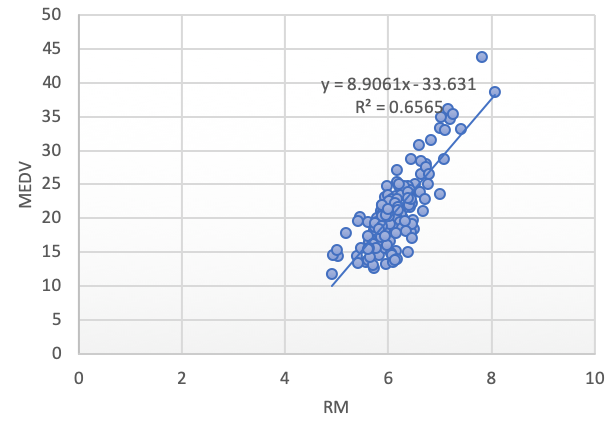
\includegraphics{part1/boston-rm.png}}
	\end{figure}

	\begin{lstlisting}[language=java]
	double []RM = {6.575, 6.421, 7.185, 6.998, 7.147, 6.43, 6.012, 6.172, 5.631};
	double []MDEV = {24, 21.6, 34.7, 33.4, 36.2, 28.7, 22.9, 27.1, 16.5};
	\end{lstlisting}

	使用最小二乘法就可得出上图的结果,在后续章节我们会逐步实现相关的算法。
	很明显二乘法没有体现任何机器学习的过程,模型和参数直接通过数学推算得来。
	而“学习”是指,计算机从已有数据缓慢逼近真实结果,通常利用梯度下降算法实现。
\end{example}
\bigskip

\begin{exercise}
	创建和初始化数组的方法有哪几种?请写出示例代码。
\end{exercise}

\begin{exercise}
	定义一个数组,表示魔方的2个状态:旋转前、旋转后。
\end{exercise}

\begin{figure}[!htb] \centering
	\begin{minipage}{0.4\textwidth}
		\centerline{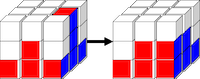
\includegraphics[scale=.5]{part1/rubik.png}}
	\end{minipage}
	\begin{minipage}{0.4\textwidth}
		\centerline{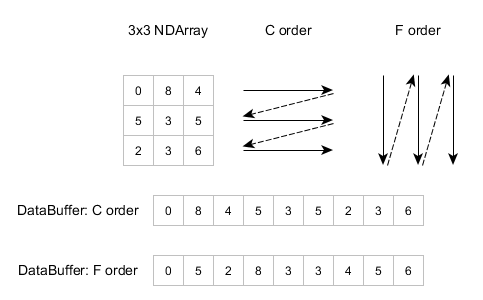
\includegraphics[trim=0 4.6cm 0 2.6cm,scale=.45, clip]{c_vs_f_order.png}}
	\end{minipage}
\end{figure}

\begin{exercise}
	如何定义矩阵(Matrix),你认为哪种方式更好?试对比行优先和列优先策略。
	\footnote{C order: 行优先;F order:列优先。}
\end{exercise}

\section{字符串}
字符串广泛存在于各种编程语言中,在Java中字符串属于对象,提供了String创建和操作字符串。
String内部维护着一个char[]数组,你也可以用char[]初始化一个String类型。
Java虽然不支持运算符重载,但字符串可以和其它类型相"+"拼接。
\medskip

\begin{lstlisting}[language=Java]
	String fullName    = "张三";
	String lastAndName = "张" + "三";

	String fullNameNew = new String("张三");
	String intern      = fullNameNew.intern();
	System.out.println ( fullName    == lastAndName ); true
	System.out.println ( lastAndName == fullNameNew ); false
	System.out.println ( fullName    == intern      ); true
\end{lstlisting}

\begin{exercise}
	请调查字符串的默认编码?
\end{exercise}

\section{集合Collection<E>}
数组创建之后不能再改变大小,删除和插入都不太方便。
Java提供了Collection<E>的多种实现:ArrayList<E>、LinkedList<E>等。
其中E是值的类型,但不能是\underline{\emph{基本}}类型。
因此,基本类型要换成相应的封装类,才能使用Collection<E>。

\begin{lstlisting}[language=Java, backgroundcolor=\color{lightgray!10}]
	jshell> ArrayList<int> ages;
	|  错误: 意外的类型
	|  需要: 引用
	|  找到:    int
	|  ArrayList<int> ages;
	|            ^-^
	jshell> ArrayList<Integer> ages;
	ages ==> null
	jshell> ArrayList<int[]> ages;
	ages ==> null	
\end{lstlisting}

\remark{
	值得注意的是,虽然int是基本类型,但int[]不是。
	基本类型不需要申请内存,放在方法栈里,而int[]是分配了一块连续内存。
}
\bigskip

实际上ArrayList是通过数组实现的,默认大小为10。
如果10个满足不了要求,最好设置一个默认长度。
因此,ArrayList继承了数组的优点(访问快)和缺点(增删不易)。
需要对频繁插入、删除操作,建议使用LinkedList。
更多Collection的知识,大家可以参照Java专门书籍深入学习。
\bigskip

\begin{example}
	基本类型的数组,要转换为对应的封装类型数组,不能强转赋值。
\end{example}
\begin{lstlisting}[language=Java]
	int[] dataInt = {1, 2, 6, 7, 9, 5, 1};
	Integer[] dataInteger = Arrays.stream(dataInt)
							.boxed()
							.toArray(Integer[]::new);
	String s = Arrays.asList(dataInteger).stream()
							.map(n->n.toString())
							.collect(Collectors.joining("-"));
  System.out.println(s);
\end{lstlisting}

\remark{这里用到Java语言的$\lambda$语法和方法,在后面章节会作简要说明。}
\bigskip

\begin{exercise}
	分析以下代码,array1和array2存在什么不同?
	\begin{lstlisting}[language=Java]
		int[] times1 = {1, 2, 6, 7, 9, 5, 1};
		Integer[] times2 = {1, 2, 6, 7, 9, 5, 1};
		List<int[]> array1 = Arrays.asList(times1);
		List<Integer> array2 = Arrays.asList(times1);
	\end{lstlisting}
\end{exercise}

\section{字典Map<K,V>}
	在Java语言中Map不是关键字,也不是基本类型,但提供了几个实现可以直接使用。
	由定义Map<K, V>,它是一个泛型类,可以存放很多类型的数据。
	其中K是关键字的类型、V是值的类型。
	典型的Map实现有HashMap、LinkedHashMap\footnote{linked串联代表着有序},
	其余的请参考其它书籍。
	与HashMap不同的是,LinkedHashMap会把插入数据的顺序记住。
	\bigskip

	\begin{lstlisting}[language=Java, backgroundcolor=\color{lightgray!10}]
		jshell> HashMap<String, Integer> hashMap = new HashMap<>();
		jshell> hashMap.put("A", 10)
		jshell> hashMap.put("C", 12)
		jshell> hashMap.put("B", 11)

		jshell> hashMap.keySet()
		$7 ==> [A, B, C]
		jshell> hashMap.values()
		$5 ==> [10, 11, 12]
		jshell> hashMap.entrySet()
		$6 ==> [A=10, B=11, C=12]
		jshell> hashMap.get("A")
		$8 ==> 10
	\end{lstlisting}

	\begin{exercise}
		修改本节代码为LinkedhashMap,再执行一遍,比较其差异。
	\end{exercise}

\section{赋值和引用}
在一些编程语言中,存在值传递和引用传递的区别。
Java中基本类型都是值传递,譬如\lstinline{a=b}之后,a和b就再无关系。
但数组和对象(如String)不是这样的,赋值之后就指向了同一个对象。

\begin{lstlisting}[language=Java, backgroundcolor=\color{lightgray!10}]
	jshell> int []age_list = {1,2,3,4};
	age_list ==> int[4] { 1, 2, 3, 4 }
	jshell> var p = age_list
	p ==> int[4] { 1, 2, 3, 4 }
	jshell> p[0]=10
	$3 ==> 10
	jshell> age_list
	age_list ==> int[4] { 10, 2, 3, 4 }
\end{lstlisting}

\begin{exercise}
	从内存的角度,如何理解值传递和引用传递?
\end{exercise}


\section{运算符}
	到这里,应当已经掌握赋值语句和声明语句,但还不能表达逻辑推理。
	算式和逻辑运算,和其它语言没有太大的区别。
	下表是Java支持的运算符和优先级。

\begin{table}[!htbp] \centering \small
	\begin{tabular}{p{4cm}|p{8cm}}
	\toprule
	运算符     & 优先级 \\
	\midrule
	单目运算符   & {\lstinline@++(前/后) --(前/后) +expr -expr ~ !@} \\ \hline
	乘、除、余   & {\lstinline@* / %@} \\ \hline
	加、减      & {\lstinline@+ -@} \\ \hline
	位移        & {\lstinline@<< >> >>>@} \\ \hline
	关系运算符   & {\lstinline@< > <= >= instanceof@} \\ \hline
	判等        & {\lstinline@== !=@} \\ \hline
	按位与      & {\lstinline@&@} \\ \hline
	按位异或    & {\lstinline@^@} \\ \hline
	按位或      & {\lstinline@|@} \\ \hline
	逻辑与      & {\lstinline@&&@} \\ \hline
	逻辑或	    & {\lstinline@||@} \\ \hline
	三目运算符   & {\lstinline@?:@} \\ \hline
	赋值        & {\lstinline@= += -= *= /= \%= &= ^= |= <<= >>= >>>=@} \\
	\bottomrule
	\end{tabular}
	\caption{Java运算符和优先级}
\end{table}
\remark{\~是数值取反,!是布尔取反。}

\subsection{算术运算}
常见的数值运算符号,在此不作介绍,需要重点关注的是递增/减运算符和逻辑运算符。
递增/减运算符放在变量前面,就会先计算再赋值;后面则是先赋值后计算。
\begin{example} ++、--运算符示例:
\begin{lstlisting}[language=Java, backgroundcolor=\color{lightgray!10}]
	jshell> var a=2
	a ==> 2
	jshell> var b=++a
	b ==> 3
	jshell> var c=b++
	c ==> 3
	jshell> var d=c--
	d ==> 3
	jshell> c
	c ==> 2
\end{lstlisting}
\end{example}

位运算,通常用于标志位检查。譬如short类型有16位可以使用,可代表16+1个状态。
下述代码检查s的第一位是否为1,检查第三位是否为1。
\begin{example}
	\begin{lstlisting}[language=Java, backgroundcolor=\color{lightgray!10}]
		jshell> short s=0b0000_0100_0011
		s ==> 67
		jshell> Integer.toHexString(s)
		$34 ==> "43"
		jshell> s & 0b0001 // 二进制以 0b 开头
		$36 ==> 1
		jshell> s & 0b0100
		$37 ==> 0
	\end{lstlisting}
\end{example}

位移,可把int/long划分成多个字节,也可以拼接为一个int/long数值。
譬如RGB颜色,包含3个部分:0xRRGGBB(十六进制)。
如果要把某图像编程灰度图像,典型的代码如下:

\begin{lstlisting}[language=Java]
	int r = (color >> 16) & 0xff;
  int g = (color >> 8) & 0xff;
	int b = color & 0xff;
	int gray = (int) (0.3 * r + 0.59 * g + 0.11 * b);
\end{lstlisting}

\remark{为什么要按位与0xff呢?数据类型哪一节作业完成了吗?}

\subsection{逻辑运算}
Java语言中,布尔类型只有2个值:\lstinline[language=Java]{true、false}。
比较运算产生布尔结果,且只有布尔值才能参与逻辑运算。
运算符\lstinline{&&},具有截断效果:

\begin{lstlisting}[language=Java, backgroundcolor=\color{lightgray!10}]
	jshell> var a = 2
	a ==> 2
	jshell> var b = 3
	b ==> 3
	jshell> b < 3 && a++ > 2 // a++被截断没有执行
	$41 ==> false
	jshell> a
	a ==> 2
	jshell> b <= 3 && a++ > 2 // b<=3成立,a++获得执行
	$43 ==> false
	jshell> a
	a ==> 3
\end{lstlisting}

\section{循环语句}
数组和字典存可存放很多数据,经常要遍历逐一取出来处理。
Java提供了四种循环结构:
\lstinline[language=Java]{for/foreach/while/do...while}语句等。
\bigskip 

\begin{table}[!htbp]\centering
	\lstset{frame=none, aboveskip=0mm, belowskip=0mm}
	\begin{tabular}{|p{6cm}|p{7cm}|}
	\hline
	\multicolumn{2}{|c|}{for语句}\\
	\hline
	\begin{lstlisting}[language=Java]
		for(初值; 布尔表达式; 步进) {
			//代码语句
		}
	\end{lstlisting}
	&
	\begin{lstlisting}[language=Java]
		// sum = 1+2+...+100
		int sum = 0;
		for (int i=1; i<=100; i++) {
			sum += i;
		}
	\end{lstlisting} \\
	\hline
	\begin{lstlisting}[language=Java]
		// 类似for...in的方式
		for(声明语句 : 表达式) {
			//代码句子
		}
	\end{lstlisting}
	&
	\begin{lstlisting}[language=Java]
		// sum = 1+2+...+9
		int[] list = {1,2,3,4,5,6,7,8,9};
		int sum = 0;
		for (int i: list) {
			sum += i;
		}
	\end{lstlisting} \\
	\hline
	\end{tabular}
\end{table}

近年来,Java也从其它语言汲取了很多改进,
所有的集合(Collection的实现)不仅可以使用\lstinline{for(:)}的方式还可以使用forEach接口遍历数据。
\bigskip

\begin{lstlisting}[language=Java]
	// 支持:数组、集合
	for(Integer i : array) {
    System.out.println(i);
	}
\end{lstlisting}

\noindent 在Java8之后,现在你可以可以写成:
\begin{lstlisting}[language=Java]
	//array.forEach(i -> System.out.print(i));
	array.forEach(System.out::print); // 已支持函数式编程
\end{lstlisting}
\bigskip

与for明显不同的是,while循环只有一个布尔表达式。
使用哪种循环表达式更好,取决于你的需要。
如果需要下标,最好还是使用for循环。

\begin{table}[!htbp]\centering
	\lstset{frame=none, aboveskip=0mm, belowskip=0mm}
	\begin{tabular}{|p{5cm}|p{8cm}|}
	\hline
	\multicolumn{2}{|c|}{while语句}\\
	\hline
	\begin{lstlisting}[language=Java]
		while( 布尔表达式 ) {  
			//代码语句
		}
	\end{lstlisting}
	&
	\begin{lstlisting}[language=Java]
			// sum = 1+2+...+100
			int sum = 0, i = 0;
			while (i <= 100) {
				sum += i;
				i++;
			}
	\end{lstlisting} \\
	\hline
	\begin{lstlisting}[language=Java]
		do {
			//代码句子
		} while(布尔表达式);
	\end{lstlisting}
	&
	\begin{lstlisting}[language=Java]
			// sum = 1+2+...+100
			int sum = 0, i = 0;
			do {
				sum += i;
				i++;
			} while (i <= 100);
	\end{lstlisting} \\
	\hline
	\end{tabular}
\end{table}
\noindent

循环语句是可以嵌套的:先进入外层循环,再进入内层循环,
然后直到内层循环条件不满足,跳出到外层循环。
如果外层循环也不满足,执行结束。
\lstinline{break}和\lstinline{continue}可以影响循环的执行顺序。
使用\lstinline{break}跳出当前循环,注意只是跳出一层。
而\lstinline{continue}是跳过一轮循环,执行下一轮。
\bigskip

\begin{lstlisting}[language=Java]
	// 计算 sum = 1+3+5+7+9
	int sum = 0;
	for (int i = 0; i <= 20; i++) {
		if (i%2 == 0) continue; // 可省略大括号
		else if (i>10) break; // 可省略大括号
		sum += i;
	}
\end{lstlisting}

实际上,使用\lstinline{break}也可以跳出多层循环,但很少使用。
需要先声明一个label,以指定\lstinline{break}跳转的位置,
它的用法有点类似于\lstinline{goto}语句等。
使用\lstinline{break}只能跳转到包含该break语句的代码块,
譬如,你不能跳转到例子中嵌套循环之前或之后的代码行上。
\bigskip

\begin{lstlisting}[language=Java]
	int[][][] ids = {
					{{1,2,3}, {10,20,30}, {100,200,300}},
					{{3,4,5}, {30,40,50}, {300,400,500}},
					{{6,7,8}, {60,70,80}, {600,700,800}}
	};

	found: 
	for (int i = 0; i < 3; i++) {
		for (int j = 0; j < 3; j++) {
				for (int k = 0; k < 3; k++) {
						if (ids[i][j][k] == 10) {
								System.out.printf("ids[%d,%d,%d]\n", i, j, k);
								break found;
						}
				}
		}
	}
	System.out.println("bye!");
	/**** 输出:*****
	ids[0,1,0]
	bye!
	****************/
\end{lstlisting}
\bigskip

\begin{example}
	计算如下2个int矩阵相加的结果,矩阵使用二维数组表示。\\
	\begin{minipage}{0.3\textwidth}
		$$
		A = \left[
		\begin{matrix}
			1 & 2 & 3 \\
			4 & 5 & 6 \\
			7 & 8 & 9
			\end{matrix}
			\right]
		$$
	\end{minipage}
	\begin{minipage}{0.3\textwidth}
		$$
		B = \left[
		\begin{matrix}
			10 & 20 & 30 \\
			40 & 50 & 60 \\
			70 & 80 & 90
			\end{matrix}
			\right]
		$$
	\end{minipage}
	\bigskip

	\noindent \emph{示例代码:}
	\begin{lstlisting}[language=Java]
		int[][] A = {{1,2,3}, {4,5,6}, {7,8,9}};
		int[][] B = {{10,20,30}, {40,50,60}, {70,80,90}};
		int[][] C = new int[3][3];

		for(int r = 0; r < 3; r++) {
			for (int c=0; c < 3; c++) {
				C[r][c] = A[r][c] + B[r][c];
			}
		}
	\end{lstlisting}

\end{example}

\begin{example}
	波士顿房价数据中,存在一些无效数据(非数值,如N/A等),要把它们剔除掉。
	假设我们读出来都是字符串:
	房间数["6.421", "NA", "6.998", "7.147", "6.43", "6.012", "6.172", "5.631"];
	房均价["21.6", "34.7", "", "36.2", "28.7", "22.9", "27.1", "16.5"];
\end{example}

\noindent \emph{示例代码:}
\begin{lstlisting}[language=Java]
	String []rooms = {
		"6.421", "NA", "6.998", "7.147", "6.43", "6.012", "6.172", "5.631"
	};
	String []values = {
		"21.6", "34.7", "", "36.2", "28.7", "22.9", "27.1", "16.5"
	};
	double []RM = new double[20];
	double []MDEV = new double[20];
\end{lstlisting}

\noindent
这里没有主动检测字符串是否为合法数字,而使用了Double提供的解析方法。
如果不能正确解析为数字,parseDouble函数就会抛出异常。
出现异常之后,我们什么都不需要做,继续下一轮解析即可。
\bigskip

\noindent \emph{示例代码:}
\begin{lstlisting}[language=Java]
	int pos = 0;

	for (int i = 0; i < rooms.length; i++) {
		try {
			double d1 = Double.parseDouble(rooms[i]);
			double d2 = Double.parseDouble(values[i]);
			RM[pos] = d1;
			MDEV[pos++] = d2;
		} catch (NumberFormatException ignored){
			// 出错了,什么都不做
		}
	}

	while (--pos >= 0) {
		System.out.printf("%.3f -> %.3f\n", RM[pos], MDEV[pos]);
	}
\end{lstlisting}

\noindent
请认真阅读以上代码,对于++/--运算符要掌握清楚!
\bigskip

\begin{exercise}
	请尝试用foreach的方式遍历rooms数组。
\end{exercise}

\begin{exercise}
	请尝试用while的2种方式遍历rooms数组。
\end{exercise}

\begin{exercise}
	使用循环实现斐波那契数列的算法:0,1,1,2,3,5,8,13,21。
\end{exercise}

\section{判断语句}
使用if语句可根据条件是否为真(true、false),选择执行不同的代码。
其中,else语句是可有可无的,写个空的\lstinline!else{}!也很常见(注意加上注释!)。
\lstinline{if}语句之后,可以有若干个\lstinline{else if}语句,但它们必须在\lstinline{else}语句之前。
具体的形式有以下几种:

\begin{table}[!htbp]\centering
	\lstset{frame=none, aboveskip=0mm, belowskip=0mm}
	\begin{tabular}{|p{6.5cm}|p{6.5cm}|}
	\hline
	\multicolumn{2}{|c|}{if语句}\\
	\hline
	\begin{lstlisting}[language=Java]
			// 只说明成立的时候做啥
			if (条件) {
					//TODO:成立做啥
			}
	\end{lstlisting}
	&
	\begin{lstlisting}[language=Java]
			// 成立和不成立
			if (条件) {
					//TODO:条件成立
			} else {
					//TODO:条件不成立
			}
	\end{lstlisting} \\
	\hline
	\begin{lstlisting}[language=Java]
			// 多个条件,都不成立啥也不做
			if (条件1) {
					//TODO:条件1成立
			} else if (条件2) {
					//TODO:条件2成立
			} else if (条件3) {
					//TODO:条件3成立
			}
	\end{lstlisting}
	&
	\begin{lstlisting}[language=Java]
			// 多个条件
			if (条件1) {
					//TODO:条件1成立
			} else if (条件2) {
					//TODO:条件2成立
			} else {
					//TODO:否则只能
			}
	\end{lstlisting} \\
	\hline
	\end{tabular}
	\caption{判断语句if-else}
\end{table}

\bigskip

\begin{example}
	结合循环和判断语句,已经可以编写很多算法。
	例如,使用随机打点法,检查落点是否在圆周内,以统计方法计算圆周率。
\end{example}

\begin{figure}[!htbp]
	\centerline{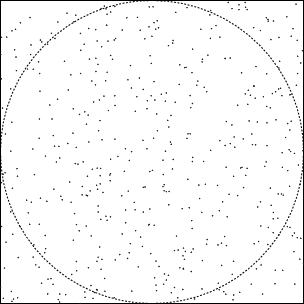
\includegraphics[scale=0.4]{part1/dot-pi.png}}
\end{figure}

\begin{lstlisting}[language=Java]
	Random random = new Random(System.currentTimeMillis());
	int total = 1_0000, hit = 0; // 数字可以用下划线分割
	double x = 0, y = 0;

	for (int i = 0; i < total; i++) {
			x = random.nextDouble();
			y = random.nextDouble();
			if (x*x+y*y < 1) hit++; // 只有一行代码的时候可以忽略大括弧
	}

	System.out.println(hit*4.0/total);
\end{lstlisting}

\section{分支语句}
当然\lstinline{if}语句包含很多\lstinline{else if}的时候,
你应当考虑是否可以优化为\lstinline{switch}或者函数表的形式。
\lstinline{swtich}语句判断条件变量是否与某个\lstinline{case}的值中是否相等,
每个值称为一个分支。

\begin{lstlisting}[language=Java]
	switch(expression){
	case value: //可以有任意数量的case语句
		//语句
		break; //可选,不加会继续与下一个case比较!
	case value:
		//语句
		break;
	default : //可选,建议经常添加
		//语句
	}
\end{lstlisting}

\noindent
switch 语句中的变量类型可以是: byte、short、int 或者 char。
从JDK7开始,switch已支持字符串类型了。
\bigskip
\remark{同时case标签必须为字符串常量或字面量。}
\bigskip

\begin{example}
	手写数字识别,最后使用10个bit位代表0-9的识别结果。
	譬如,0000000001就代表识别结果为数字1。
\end{example}

\begin{lstlisting}[language=Java]
	int ret = 1 << 5;
	switch(ret) {
		case 0b00000_0000: System.out.println("0");break;
		case 0b00000_0001: System.out.println("1");break;
		case 0b00000_0010: System.out.println("2");break;
		case 0b00000_0100: System.out.println("3");break;
		case 0b00000_1000: System.out.println("4");break;
		case 0b00001_0000: System.out.println("5");break;
		case 0b00010_0000: System.out.println("6");break;
		case 0b00100_0000: System.out.println("7");break;
		case 0b01000_0000: System.out.println("8");break;
		case 0b10000_0000: System.out.println("9");break;
		default: System.out.printf("NA, %d", ret);
	}
\end{lstlisting}

\section{异常处理}
在一些语言中,处理错误就是检查返回值。
而Java提供了\lstinline!try{代码}catch{异常处理}finally{兜底代码}!。
有些函数会明确自己会抛出异常(throws、throw),
如果不是运行时异常,就必须得编写异常处理语句。
异常被\lstinline{catch}捕获,就跳转执行异常处理代码,
而finally代码块无论是否发生异常都会被执行。
\medskip
\begin{lstlisting}[language=Java]
	try {
		// 正常代码
	} catch(XxxException e) { 
		// 捕获到的异常,还可以重写抛出
		throw e; // 再次抛出
	}
 
	try {
		// 正常代码
	} catch(XxxException e) {
		// 异常处理代码
	} finally { 
		// 先try语句,再catch语句,最后finall语句,无异常也会执行finally
	}
 
	try {
		// 正常代码
	} finally { 
		// 有没有异常不关心,但出现异常之后我有机会先执行
	}
 
	try {
		// 正常代码
	} catch(XxxException e) { 
		// 多个异常类型,可以合并为一个catch语句
	} catch(XxxException e) { 
		// 存在继承关系的情况,子类放在前面,并且不能使用|合并
	}
 \end{lstlisting}

\section{定义函数}
程序的三个特征:有限步之后可退出;有0个或多个输入;有一个或多个输出。
使用函数不仅可以把特定功能的代码打包在一起,还便于重用代码。

\begin{definition}{函数}{func}
	修饰符 \textvisiblespace 返回值类型 \textvisiblespace 方法名\(参数类型 参数名\) \{ \\
  \codeident[1cm] $\dots$ \\
  \codeident[1cm] 方法体 \\
  \codeident[1cm] $\dots$ \\ 
  \codeident[1cm] return 返回值; \\
	\}
\end{definition}

\noindent
方法的名字的第一个单词应以小写字母作为开头,后面的单词则用大写字母开头写,不使用连接符。
修饰符是可选的,影响函数的调用方法和范围,定义了该方法的访问类型。
返回值return,也是可选的。
如果没有返回值,可去掉return,并把返回值类型改成void。
\bigskip
\begin{lstlisting}[language=Java, backgroundcolor=\color{lightgray!10}]
	jshell> double piByProbability(int total) {
   ...>         Random random = new Random(System.currentTimeMillis());
   ...>         int hit = 0;
   ...>         double x = 0, y = 0;
   ...> 
   ...>         for (int i = 0; i < total; i++) {
   ...>                 x = random.nextDouble();
   ...>                 y = random.nextDouble();
   ...>                 if (x*x+y*y < 1) hit++;
   ...>         }
   ...> 
   ...>         return hit*4.0/total;
   ...>     }
|  已修改 方法 piByProbability(int)
jshell> piByProbability(10000);
$8 ==> 3.1464
jshell> piByProbability(1000000000)
$17 ==> 3.141672248
\end{lstlisting}

\noindent
函数也可以自己调用自己,称为迭代。
这有点类似于数学迭代公式:$f_n(x) = f_{n-1}(x)*n$。

\bigskip
\begin{exercise}
	使用迭代,实现求n!的函数。
\end{exercise}

\begin{exercise}
	使用迭代,实现求斐波那切数列的函数,输出前10个数字。
\end{exercise}

\section{Java对象}
对象是对代码的一种编写方式,即使是C语言也可以使用类似的机制。
它的好处在于把相关的代码和数据封装一起,并且可以限制外部对其数据和函数的访问。
同时,对象作为一个母版刻画了一个类型应该具有的属性和方法(函数在对象内称为方法)。

实际上,Java语言是不允许函数独立存在的,只能放在某个对象类型里面。
jshell比较特殊,可以快速验证代码。
面向对象编程涉及到的理论知识非常多,本书不作过多介绍。
继承,是面向对象的核心,可理解为一种代码复用扩展的方法。

\begin{definition}{类和接口}{class}
	\lstinline@[修饰符] interface 接口 { @ \\
	\lstinline@	常量和方法声明@ \\
	\lstinline@}@ \\
	\lstinline@[修饰符] class 父类 { @ \\
	\lstinline@	属性和方法@ \\
	\lstinline@}@ \\
	\lstinline@[修饰符] class 子类 extends 父类 implements 接口 {@ \\
	\lstinline@	子类的属性和方法,要实现接口方法@ \\
	\lstinline@}@
\end{definition}

访问修饰符,可加在类、属性、函数(包括构造函数)的前面,用于限制其可见性。
减少对外的可见性,能提供代码的灵活性。
总之,对外提供功能减少细节暴露,可防止以后修改内部实现,导致牵一发而动全身的问题出现。

\begin{table}[!htbp]\centering
	\begin{tabular}{|p{3cm}|p{1.6cm}|p{1.6cm}|p{2cm}|p{2.4cm}|}
	\toprule
	\multicolumn{5}{|c|}{Java访问权限}\\ 
	\midrule
	&同一个类&同一个包&不同包子类&不同包非子类\\ \hline
	private&$\surd$&&&\\ \hline
	public&$\surd$&$\surd$&&\\\hline
	protected&$\surd$&$\surd$&$\surd$&\\ \hline
	缺省(package)&$\surd$&$\surd$&$\surd$&$\surd$\\
	\bottomrule
	\end{tabular}
\end{table}

\begin{lstlisting}[language=Java]
	public class Vector{}  // 向量
	public class Martrix{} // 矩阵
\end{lstlisting}

\section{定义向量}

\section{定义矩阵}

\section{导数运算}

\section{梯度下降}

\section{线性回归}
